%%%%%%%%%%%%%%%%%%%%%%%%%%%%%%%%%%%%%%%%%%%%%%%%%%%%%%%%%%%%%%%%%%%%%%%%%%%%%%%%%%
%%																				%%
%% File name: 		00sarah.tex													%%
%% Project name:	Hochleistungsantenne										%%
%% Type of work:	T3X00 project work											%%
%% Author:			Sarah Brückner, Maximilian Stiefel, Hannes Bohnengel		%%
%% Date:			27th Arpil 2016												%%
%% University:		DHBW Ravensburg Campus Friedrichshafen						%%
%% Comments:		Created in gedit with tab width = 4							%%
%%																				%%
%%%%%%%%%%%%%%%%%%%%%%%%%%%%%%%%%%%%%%%%%%%%%%%%%%%%%%%%%%%%%%%%%%%%%%%%%%%%%%%%%%
%\cite{kauffels}\newpar

\chapter{Projektmanagement}
Schon Thomas Carlyle (1795–1881) erkannte die Wichtigkeit von strukturierten und organisiertem Vorgehen als er sagte:\newpar
``Unsere Hauptaufgabe ist nicht, zu erkennen, was unklar in weiter Entfernung liegt, sondern zu tun, was klar vor uns liegt''.\newpar
In einem Projekt ist das strukturierte und ogranisierte Vorgehen der klare Weg zu einem erfolgreichem Ziel. Daher wird sich in dieser Arbeit
dem Projektmanagement bedient um die Antennennachführung für Satelliten in die richtige Richtung zu lotzen. Dabei lehnt sich das Management an 
das bekannte V-Modell, welche den Abflauf von Software-, als auch von Hardwareentwicklungsprozessen beschreibt. Dieses Modell soll einem Projekt 
die Richtung weisen, jedoch werden die einzelnen Schritte vom Projektmanager selbst definiert. Ein Vorgehensmodell wie dieses legt folgende
Prozesse fest:
\begin{itemize}
 \item die Aktivitäten die durchzuführen sind,
 \item die Reihenfolge des Arbeitsablaufes,
 \item die Definition von Ergebnissen,
 \item die Fertigstellungskriterien,
 \item die Ressourcen die vorhanden sind
 \item und die anzuwendenden Standards/Werkzeuge.
\end{itemize}
\begin{figure}[h]
 \centering
 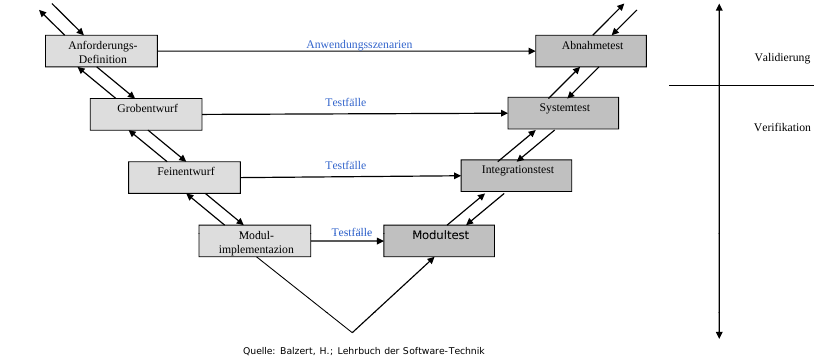
\includegraphics[width=0.8\linewidth]{./images/vmodell}
 \caption{V-Modell, Quelle: Universität Leipzig, Softwaretechnik}
 \label{fig:vmodell}
\end{figure}
Eine wichtige Rolle spielt die Qualitätssicherung, die das V-Modell sicher stellt. In diesem Modell sind die Verifikation und die Validation ein 
fester Bestandteil. Verifikation bedeutet, die Sicherstellung dass das entwickelte Produkt mit den Spezifikationen übereinstimmt.
Die Validation ist die Eignung des Produkts bezogen auf seinen Einsatzzweck. Durch die Sicherstellung beider Qualitätsmerkmale wird das Projekt 
erfolgreich zu seinem Ziel, die Antnennennachführung für Satelliten, geführt.Aus diesem Grund ist das V-Modell die richtie Vorangehensweise für 
dieses Projekt.\newpar

\section{Zeitplan}
\section{Anforderungsdefinition}
\section{Arbeitspakete}




